\chapter{Experiments and Results}
\label{cha:ResearchAndResults}

{\it In this chapter, the results from the experiments will be presented and discussed. Section \ref{sec:results} contains the actual results created by running each scenario. The setup of the experiment is explained in section \ref{sec:experimentalSetup} explains the setup and which parameters have been used to run the experiments.
Section \ref{sec:discussion} will discuss the results seen in section \ref{sec:results}, and a discussion on the differences between the results from the simulator and the physical robots.}

\section{Experimental Plan}
\label{sec:experimentalPlan}

The results are created by writing to a text file in the form of a .csv file, which can be open directly by spreadsheet softwares. A .csv file is simply a text file with comma separated values, a row in the .csv file would correspond to a row in the spreadsheet, and a column in the spreadsheet software is separated by a comma in the .csv file.

The watcher software have no way to find the actual velocity of the robots, because the wheels still move when the robot is turning on the same spot. We want to find out if the position of each robot have changed over a given time interval.
The way the watcher software calculates the velocity of each robot is to save the old position of the robot, then compare it with the new position and see how far off it is.
The formula used to find the mean value of all the robots at a time step is defined as:
\begin{equation}
\label{eq:muvel}
\mu_{velocity} = \frac{1}{N} \Sigma_{i=1}^N (P_{i_{new}} - P_{i_{old}})
\end{equation}

where:
\\
$p_{i_{new}}$ = the new updated position of the robot
\\
$p_{i_{old}}$ = the old position of the robot from last time step
\\
$N$ = number of robots used, in this experiment $N = 4$ 
\\
$\mu_{velocity}$ = the mean of the velocities in that time step

The average distance seen in section \ref{sec:results} are calculated the same way for both the physical experiment and in the simulator. Each entity's position is found and compared with the position of all the other entities. The length of the distance between each of them are used to find the average and the standard deviation.
The formula to find 

\begin{equation}
\mu_{distances} = \frac{1}{ {N \choose R}} \Sigma_1^{N \choose R} | P_x - P_y |
\end{equation}

where:
\\
$P_x$ = the position of robot x, and $x \neq y$
\\
$P_y$ = the position of robot y, and $x \neq y$
\\
$N$ = the number of robots or Boids used
\\
$R$ = the amount of entities that are being compared each time, in this experiment we only measures the distance between two entities at the same time, therefore $R = 2$.
\\
$N \choose R$ = the combination operator, this corresponds to $ \frac{N!}{R! (N-K)!}$
\\
$\mu_{distances}$ = the mean of the compared distances in that time step
\\

The same procedure was applied for the angle of each entity: 
\begin{equation}
\mu_{angles} = \frac{1}{ {N \choose R}} \Sigma_1^{N \choose R} | A_x - A_y |
\end{equation}
where:
\\
$A_x$ = the angle of robot x, and $x \neq y$
\\
$A_y$ = the angle of robot y, and $x \neq y$
\\
$\mu_{angles}$ = the mean of the compared angles in that time step.
\\

To find the standard deviation of the velocity, the formula in equation \ref{eq:sd} was used, but a modification was done for the standard deviation of the distances and angles as seen in equation \ref{eq:sd2} because we had $ {N \choose R}$ number of distances and angles. The reason for $ {N \choose R}$ number of distances is because this is the number of comparisons between each robot. For these experiments, $N = 4$, and $R = 2$ because there is a comparison between two robot at the same time.


\begin{equation}
\label{eq:sd}
\sigma =  \sqrt{\frac{1}{N}\Sigma(X-\mu)^2}
\end{equation}

\begin{equation}
\label{eq:sd2}
\sigma =  \sqrt{\frac{1}{{N \choose R}}\Sigma(X-\mu)^2}
\end{equation}

%from template: Trying and failing is a major part of research. However, to have a chance of success you need a plan driving the experimental research, just as you need a plan for your literature search. Further, plans are made to be revised and this revision ensures that any further decisions made are in line with the work already completed. The plan should include what experiments or series of experiments are planned and what question the individual or set of experiments aim to answer. Such questions should be connected to your research questions so that in the evaluation of your results you can discuss the results wrt to the research questions.  

\section{Experimental Setup}
\label{sec:experimentalSetup}
In this section, the setup for the experiment will be explained, and which parameters have been used to run the experiments.

In this experiment, four robots and one obstacle is used inside a sandbox. Each robots needs to have an extra layer on top of them so the red and green post it note does not fall off.
In the simulator, the following parameters have been used:
\begin{description}
\item[cohesion distance] = 250 px
\item[alignment distance] = 175 px
\item[separation distance] = 120 px
\item[away from wall distance] = same as alignment
\item[obstacle distance] = same as separation
\end{description}
This distances tells the Boid how near it has to be before it should calculate the vector. For example if the Boid is in the middle of the screen, that means that it is not near a wall, then the "away from wall" function will return the null vector because it does not need the Boid to steer away from the wall.
The numbers given over is the furthest distance that the Boid will consider, for instance a Boid that have three neighbors, where one of them is 100 px away, the second one is  while the third one is 300 px away. The first Boid will be taken into consideration when calculating all of the three behaviors; cohesion, alignment and separation because it is very close. The second Boids will not have any influence on the separation behavior, but it will influence the alignment and cohesion vector. The third one is too far away, and will be ignored when calculating the three behaviors. These distances are illustrated in figure \ref{fig:simulatordistances}.

The Boids in the simulator had a velocity cap of 30 px in both x and y direction. 
The size of the robot is set to be 50 px in diameter.

Each vector from each behavior is multiplied with a factor that determines how much impact that vector will have on the final acceleration vector.
The list provided below is the weight multiplied by the behavior vector. Or $W_x$ found in equation \ref{eq:vecsum}.
\begin{description}
\item[cohesion] vector is multiplied by 2
\item[alignment] vector is multiplied by 2
\item[away from wall] vector is multiplied by 2
\item[avoid obstacles] vector is multiplied by 3
\item[separation] vector is multiplied by 3
\end{description}

As seen in the list above, the two vectors that have the highest influence on the robot is the separation and the obstacle avoidance behavior. These two behaviors needs to influence the robot a lot more than the other behaviors because they are only activated when the robot is very close to another robot or an obstacle.

The robots on the other hand had different parameters for their behaviors:
\begin{description}
\item[cohesion distance] = 800 px
\item[alignment distance] = 200 px
\item[separation distance] = 150 px
\item[away from wall distance] = same as alignment
\item[obstacle distance] = same as separation
\end{description}

The reason the cohesion distance for the physical robot are so different than the one in the simulator is because the robots are slow to flock together and they might get stuck at a corner when the sensors, so a big cohesion distance makes the robots flock together faster. The Boids in the simulator do not need the big cohesion distance because they wander a lot around even if there is no neighboring Boids around them. When they have wandered around for a while, they will eventually find another Boid that is near enough and they will start to flock together.

The simulator was intended to handle a lot more than the four Boids used in this project. If the Boids have a longer cohesion distance, more Boids would flock together and the sub flock emergence would not occur as much as seen in figure \ref{fig:subflock}.

The weights on the behavior vectors for the robots are a little bit different than the one found in the simulator.
\begin{description}
\item[cohesion] vector is multiplied by 2
\item[alignment] vector is multiplied by 2
\item[away from wall] vector is multiplied by 1
\item[avoid obstacles] does not exist
\item[separation] vector is multiplied by 4
\end{description}

The reason the avoid obstacle vector does not exist, is because the watcher software can not find nor distinguish obstacle from the floor. This feature is not implemented in the camera tracking software. The robot needs to know the size of the sandbox beforehand, because the camera or the watcher software do not provide this information to the robot. To compensate for the lack of obstacle information, the robot uses their distance sensors to find out where the obstacle are located and avoids them.

The separation vector is multiplied with a weight of 4 for the robot, but only multiplied with a weight of 3 for the Boids. There is no specific reason for this, after testing it seems to perform better with a weight of 4 on separation instead of 3.
With a weight of 3 on separation the Robots bumped into each other quite often, that is why the weight for the separation have been increased to 4.

The camera used in this experiment is a web camera. To be able to get a clear stable video feed images from the web camera, the settings for the camera had to be manually set up.
The most important setting is to disable auto focus. Auto focus makes the images blurry, and the camera tracking software will not be able to detect red and green colors which defines the robots. 50 Hz power line frequency was used instead of 60 Hz to eliminate flickering on the camera feed. The other settings are not that important, as long as the web camera is able to provide a decent looking image that the camera tracker software is able to recognize.



%The experimental setup should include all data - parameters etc, that would allow a person to repeat your experiments. 


\section{Results}
\label{sec:results}

The Boids algorithm are supposed to keep the robots flocked together and preferably they should face the same direction as well. The watcher knows where each robot is, and it knows which direction each robot is facing. The watcher measures the distance between each robot and the angle difference between the robots every five frame or twelve times each second, it then calculates the mean and standard deviation of the distances and angles and saves it to a file. The mean and standard deviation of the velocity is recorded as well, in the simulator the velocity is measured directly by getting the velocity vector on each object, for the physical robot, the change in position is measured instead.

To keep the data as consistent between each run the watcher stops all the robots and saves the data file exactly three minutes or 180,000 milliseconds after the robots have started to move.
The distance measured are in pixels. The measurement of the sandbox is 151.6 cm wide and 123.9 cm long. The watcher software creates a window that has a resolution 800x652 pixels, which means that 1 cm is approximately 5.3 pixels on the screen. The measured angles are shown in radians.

In the upcoming figures, the results from the various runs will be shown. On the x-axis the time will be shown, and the y-axis displays various types of data is presented depending on the figure. The time shown on the x-axis displays the iteration, and not seconds. One iteration takes about five frames, the software runs with a 60 frames per second. Which means that twelve iterations on the x-axis corresponds to one second. The velocity is measured every iteration, the velocity graphs is mostly used as an indication to whether the robots are moving or not. The velocity graph are able to show that the flock is moving faster or slower on certain iterations, but it can not be used to measure how fast the flock is actually moving.

\subsection{Results from scenario 1}
\label{sec:res1}

\begin{figure}[h]
\begin{center}
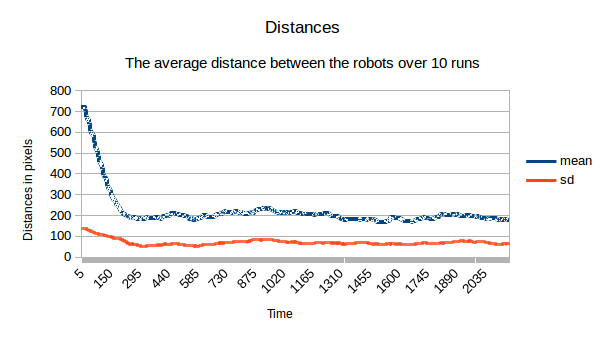
\includegraphics[width=1.1\linewidth]{figs/resdistancescene1.png}
\end{center}
\caption[Results 1]{Results from 10 runs on scenario 1}
\label{fig:scene1res}
\end{figure}

The first scenario where all the robots/Boids are placed in each corner with only one obstacle in the middle of the sandbox as seen in figure \ref{fig:scenario1}. 
These results takes the velocity by calculating $\mu_{velocity}$ by using the equation \ref{eq:muvel}, then each one is added together and averaged to create the result seen above. 

\begin{figure}[H]
    \centering
    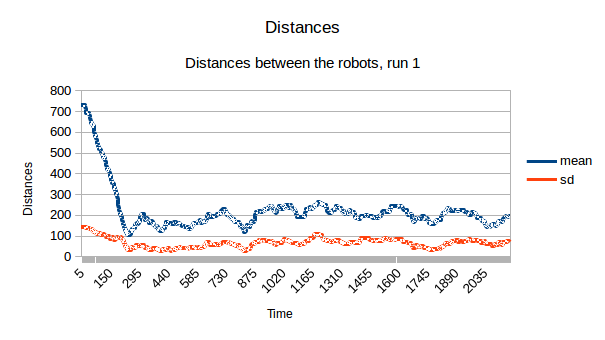
\includegraphics[width=\textwidth]{figs/scenario1_run1/dist.png}
    \caption[Distances]{Distance differences of scenario 1, run 1}
    \label{fig:distance11}
\end{figure}
\begin{figure}[H]
    \centering
    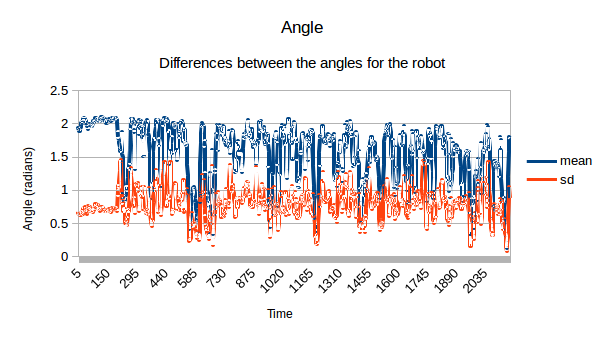
\includegraphics[width=\textwidth]{figs/scenario1_run1/angle.png}
    \caption[Angles]{Angle differences of scenario 1, run 1}
    \label{fig:angle11}
\end{figure}
\begin{figure}[H]
    \centering
    \begin{subfigure}[b]{0.4\textwidth}
        \centering
        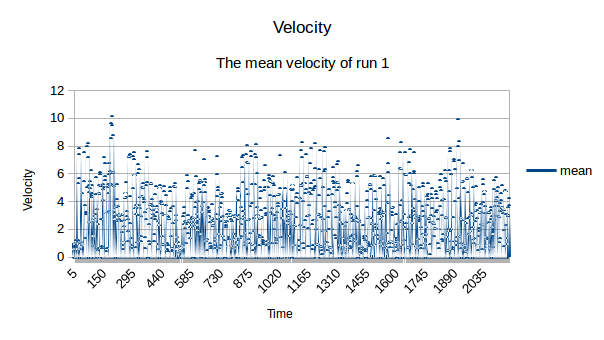
\includegraphics[width=\textwidth]{figs/scenario1_run1/velmean}
        \caption{Mean of the velocities}
        \label{fig:velmean1_1}
    \end{subfigure}
    \hfill
    \begin{subfigure}[b]{0.4\textwidth}
        \centering
        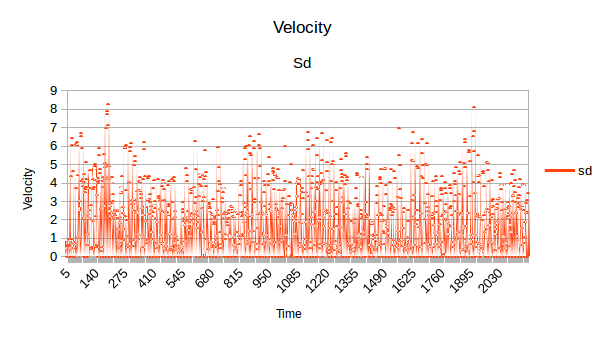
\includegraphics[width=\textwidth]{figs/scenario1_run1/velsd}
        \caption{standard deviation of velocities in scenario 1, first run}
        \label{fig:velsd1_1}
    \end{subfigure}
    \caption[Velocity]{Velocity of scenario 1, run 1}
    \label{fig:vel11}
\end{figure}
These data shown in figure \ref{fig:distance11}, \ref{fig:angle11} and \ref{fig:vel11} taken from the first run. The data from the first run is chosen to be displayed here by a random number generator.





\subsection{Results from scenario 2}
\label{sec:res2}
The second scenario in figure \ref{fig:scenario2}

\begin{figure}[h]
\begin{center}
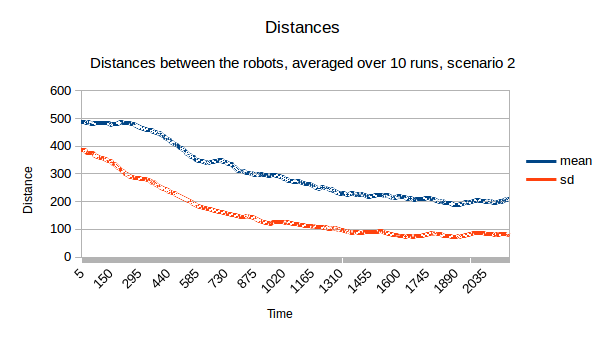
\includegraphics[width=1.1\linewidth]{figs/resdistancescene2.png}
\end{center}
\caption[Results 2]{Results from 10 runs on scenario 2}
\label{fig:scene2res}
\end{figure}

\subsection{Results from scenario 3}
\label{sec:res3}
\begin{figure}[h]
\begin{center}
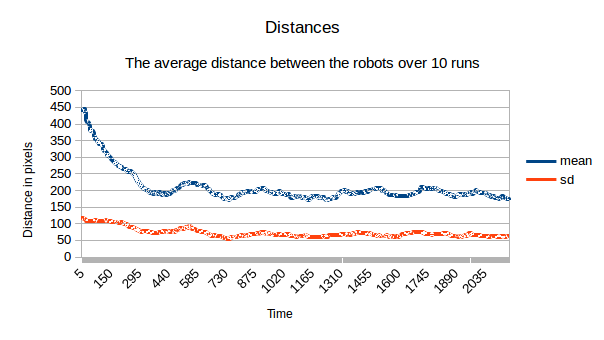
\includegraphics[width=1.1\linewidth]{figs/resdistancescene3.png}
\end{center}
\caption[Results 3]{Results from 10 runs on scenario 3}
\label{fig:scene3res}
\end{figure}
The third scenario in figure \ref{fig:scenario3}

%TODO graphs and interpretation of results
%The graph below shows

%All the graphs that was generated during the experiment can be found in the appendix.
\section{Discussion}
\label{sec:discussion}
This section will mainly focus on explaining the data from the results, why there is a difference between the physical experiment and the experiments done in a simulator.

From the results we can see that the robots quickly flock together, they start out on each corner of the sandbox then drive into the center of the sandbox, this is shown in the graph by the first drop from 700 px to around 200 px. This corresponds to roughly 132 cm to 37 cm. The time it takes for the graph to drop from 700 px to 200 px is around 300 iterations, which equals 25 seconds.

The distances converges to 200 px in about 300-400 time steps for the first scenario and the third scenario. It takes a bit longer for the distance to drop to 200 px in the second scenario, around 1310 time steps, which is approximately 110 seconds.

In the first and third scenario, each robot starts alone. Due to this, only the sensors used for obstacle avoidance, the "away from wall" and the cohesion behavior will be active. This makes each of the robot move towards the other ones, this makes the robots converge to a flock faster. 

In the second scenario, three of the robots are already in a flock while the fourth one is astray from the flock on the other side of the sandbox. The three robots that have already flocked together will try to stay together, they do not want to move all the way to the other side to flock with one single robot. If all of the robots were moving, the single robot would move towards the three robots and they all would together faster.
When running scenario 2 on the simulator, the Boids move towards the obstacle and around it. When they are near enough to the non-moving Boids, the cohesion behavior will activate and the Boids will try to flock, but due to all the other behaviors, the three moving Boid will be pushed away. After being pushed away, they will keep moving in the same direction and move all the way around the screen.

The angles measured seems to vary a lot, even if the alignment behavior tries to make all the robots face the same way. The reason this happens is because the allowed space to travel is not infinite and the robots encounters different types of obstacles like the surrounding wall, the other robots and the water bottle obstacle placed inside the sandbox. The same behavior is found on the Boids that were ran exclusively on a simulator. 

Whenever the robots detects an obstacle or move towards the walls, the distance sensors will make the robot turn around so the robot will not crash. Sometimes the robots will think that the other robots around itself are obstacles as well, because it has no way to tell the difference between the robots from an actual obstacle. This is because the distance sensors can not distinguish anything, it only measures a distance and the robots will try to avoid anything that is too near it, thinking that it sees an obstacle.

%TODO check if true
The velocity also varies a lot, going from 0 to %TODO.
The Boids in the simulator never stops, that is the velocity never drops down to 0, they keep moving in different direction all the time. Being able to move freely in all 360\textdegree\ almost instantly. They do not need to stop to change direction.
The physical ChIRP robot needs to turn around before moving in a new direction. As long as the new direction is off by an angle larger than 1\textdegree\ from the angle the robot is currently facing, then it will stop and turn. All turning takes approximately one second, before the robot is moving again. If the robot will turn a lot, it will only have one second to do so, before it has to move. If it only needs to turn 2\textdegree, it will turn first and wait until it has been one second before moving on.
The one second delay is introduced to keep the timing somewhat synchronous between the robots, one second delay is long enough for the robot to be able to almost turn all the way around (180\textdegree). 

Whenever the robot turns, the watcher will not see any change in position, which is the method it uses to log the velocity of the robots. The watcher will therefore log that the velocity of the robot is 0 when the robots turn around on the same spot. 

The graphs only shows the average distance between the robots, the velocity of the robots and the difference between their angle. The graphs do not show where the robots are moving or whether they have crashed into anything.
Sometimes the robots do bump into the obstacles, or the other robots. The reason is that the robots measures the distances before moving, and not continuously while moving. So if a robot measures the distance in front of it and there is no obstacle in front of it, it will start to move forward. When the robot moves forward it might hit an obstacle or robot if the object is too close to it when it measures the distance. Sometimes robots moves onto the path of another robot while the other robot is moving, the other robot will probably bump into the one blocking its path. 

The distance measured might be imprecise, due to disturbances around that makes the distance imprecise. The disturbances can come from the infrared light the other robots sends out when they are measuring distances themselves, which might bounds around in the sandbox and disturb the other robots.

For the camera to see the two colored post it notes on the robots, the room needs to be well lit. Extra lights were placed around the sandbox to lit it up. The room where the experiment took place had two large windows, by daytime the sun would shine into the room. The sunlight contains infrared light, if the sun shines into the room and hits the area where the robots roam, the robot will sense the infrared lights from the sunshine and think that there is an object in front of it. The blinds in the room were closed, but some sun would always shine into the room.

The robots only move forward, and they only turn when they need to change direction or if there is an object in front of it that it needs to avoid. Sometimes the robots suddenly stops and rotates on the spot as if there is some sort of object in front of it, even if there is none.